\section{Robot Localisation}
\label{sec:robot-localisation}

Robot localisation is the process of estimating a robot's pose (position and orientation) within a given reference frame using sensory information. It is a prerequisite for all navigation and manipulation tasks that require interaction with the physical environment, and is tightly coupled with mapping; together they constitute Simultaneous Localisation and Mapping (SLAM)~\cite{ullahMobileRobotLocalization2024,leonardSimultaneousMapBuilding1991}.

This section traces the historical foundations of robot localisation, structured around three persistent challenges that have shaped the field and that remain directly relevant to the methods presented in this thesis. The first is the accumulation of pose error under dead reckoning, which motivates a probabilistic treatment of uncertainty. The second is the need to represent and fuse uncertain, heterogeneous sensor measurements into a coherent spatial model. The third is the tension between short-range alignment and global map consistency. The foundational contributions reviewed here (probabilistic uncertainty modelling~\cite{smithRepresentationEstimationSpatial1987}, occupancy-based sensor fusion~\cite{elfesUsingOccupancyGrids1989}, the Iterative Closest Point (ICP) algorithm~\cite{beslMethodRegistration3D1992a}, and pose graph optimisation~\cite{luGloballyConsistentRange1997}) constitute the algorithmic backbone of the SLAM system developed in \cref{chap:SLAM} and the precise-alignment pipeline described in \cref{chap:precise-alignment}.

\subsection{The Limits of Deterministic Localisation}
\label{subsec:deterministic-localisation}

The first mobile robots capable of autonomous reasoning operated under deterministic models: each commanded action was assumed to execute perfectly, and the robot's pose was updated accordingly. Shakey the Robot (1966--1972) localised through discrete semantic labels and open-loop dead reckoning, with landmark correction that depended on the environment conforming exactly to a pre-modelled structure~\cite{nilssonShakeyRobot1984}. Moravec's Stanford Cart extended this to geometric localisation via stereo vision, maintaining explicit 3D feature positions but associating no uncertainty with them; errors accumulated silently, requiring approximately five hours for a 20-metre indoor traverse~\cite{moravecObstacleAvoidanceNavigatio1980,moravecStanfordCartCMU1990}.

These systems illustrate the core failure mode of deterministic localisation: uncorrected motion errors compound over time, and landmark-based correction is unreliable whenever the observed environment departs from assumed models. In semi-structured outdoor environments such as vineyards, where plant geometry changes seasonally, features repeat along rows, and no guaranteed prior map exists, this fragility is not a boundary case but the normal operating condition. The response was to replace deterministic pose estimates with probabilistic representations that could explicitly track and propagate uncertainty.

\subsection{Uncertainty Representation and Sensor Fusion}
\label{subsec:uncertainty-sensor-fusion}

The shift to probabilistic localisation was formalised by Smith and Cheeseman~\cite{smithRepresentationEstimationSpatial1987}, who proposed representing each spatial relationship as an \textit{approximate transformation}: a pose estimate paired with a covariance matrix encoding second-order uncertainty. Their framework introduces two fundamental operations. \textit{Compounding} propagates uncertainty through sequential transformations: when two uncertain poses are composed, the resulting covariance grows as a function of both input uncertainties, formalising what Shakey and the Cart demonstrated empirically: drift accumulates with each successive motion. \textit{Merging} reduces uncertainty by fusing independent estimates of the same quantity via a minimum-variance weighted combination, yielding a posterior covariance smaller than either input.

In a subsequent paper, Smith, Self, and Cheeseman extended this framework to the Stochastic Map~\cite{smithEstimatingUncertainSpatial2013}, in which robot and landmark poses are jointly maintained in a single state vector, the formulation underpinning Extended Kalman Filter (EKF) SLAM.

Building on this probabilistic foundation, Elfes introduced occupancy grids~\cite{elfesUsingOccupancyGrids1989}: a spatial representation in which each cell of a tessellated lattice maintains a probabilistic occupancy estimate, updated incrementally from raw sensor data through an explicit sensor model. A key insight is that individual sensor modalities carry complementary uncertainty profiles: sonar provides low range uncertainty but poor angular resolution, while stereo cameras offer good angular resolution but depth uncertainty that grows with distance. Representing both in a common occupancy-grid format allows them to be fused into a map with lower aggregate uncertainty than either source alone, as illustrated in \cref{fig:occupancyGridSensorFusion}.

Elfes also noted that fusing sensor views into a coherent global map requires accurate motion estimation, since dead-reckoning uncertainty compounds in precisely the manner formalised by Smith and Cheeseman. This co-dependence between localisation accuracy and map quality is the defining characteristic of SLAM, and directly motivates the choice in \cref{chap:SLAM} to fuse LiDAR odometry with an inertial measurement unit (IMU) whose complementary error characteristics reduce drift under the same merging principle.

\begin{figure}
    \centering
    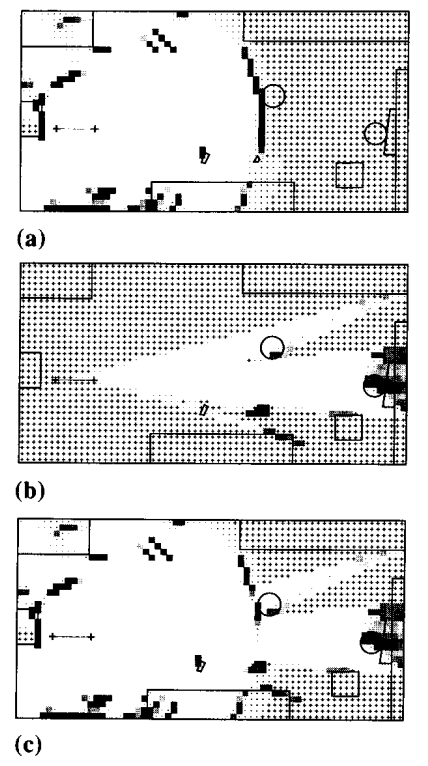
\includegraphics[width=0.5\linewidth]{2-background/figures/OccupancyGridSensorFusion.png}
    \caption{Sensor integration of sonar and scanline stereo. Occupancy grids generated separately for sonar (a) and scanline stereo (b), as well as the integrated map (c) obtained through sensor fusion, are shown. Occupied regions are marked by shaded squares, empty areas by dots fading to white space, and unknown spaces by + marks \protect\cite{elfesUsingOccupancyGrids1989}. }
    \label{fig:occupancyGridSensorFusion}
\end{figure}

\subsection{Point Cloud Registration}
\label{subsec:point-cloud-registration}

Relative pose estimation between sensor frames requires a method for aligning observations acquired at successive robot positions. Besl and McKay's Iterative Closest Point (ICP) algorithm~\cite{beslMethodRegistration3D1992a} frames registration as an optimisation problem: starting from an initial alignment, it alternates between assigning each source point to its nearest neighbour in the target cloud and solving for the rigid transformation that minimises the mean squared distance over all correspondences. Monotonic convergence of the cost function is guaranteed; however, the solution is sensitive to initial conditions and requires sufficient geometric overlap between the two clouds. Subsequent variants, notably point-to-plane error metrics~\cite{chenObjectModelingRegistration1991} and the probabilistic Generalised-ICP formulation~\cite{segalGeneralizedICP2009}, improved convergence speed and robustness in environments lacking strong planar structure.

ICP is the direct registration engine used in the precise-alignment pipeline described in \cref{chap:precise-alignment}, where a real-time point cloud of a physical vine is aligned against the SfM-derived reference geometry extracted from a 3D Gaussian Splatting model. The sensitivity of ICP to initialisation and partial overlap is a central practical constraint addressed in that chapter.

\subsection{Pose Graph Optimisation and Global Consistency}
\label{subsec:pose-graph-optimisation}

Probabilistic uncertainty modelling and local scan matching together support accurate short-range pose estimation, but do not address a deeper limitation: errors accumulated along a long trajectory cannot be corrected retroactively by filtering methods. EKF-based SLAM incorporates past measurements into a sufficient statistic and then discards the raw observations; over extended trajectories, linearisation errors accumulate and the filter becomes internally inconsistent, with different regions of the map updated independently and unable to be reconciled.

Lu and Milios addressed this by introducing pose graph optimisation~\cite{luGloballyConsistentRange1997}. In a pose graph, each estimated robot pose is a node, and each relative spatial constraint (derived from scan matching or odometry) is an edge. The optimisation objective is to find the configuration of all nodes that best satisfies the full set of edge constraints simultaneously. Because the entire history of pose estimates is retained, a single loop-closure detection event can propagate corrections backward through the trajectory, recovering a globally consistent map. The fundamental contrast with filtering is that past states are not discarded: global consistency is achieved through a batch optimisation rather than a recursive update, at the cost of a more demanding solve.

For long traversals through vineyard rows, where cumulative drift along the row axis would otherwise render multi-row maps geometrically inconsistent, this distinction is operative. The SLAM system presented in \cref{chap:SLAM} employs pose graph optimisation as its back-end, enabling loop-closure corrections to enforce global consistency across traversals of multiple vineyard rows.

\subsection{Summary}
\label{subsec:robot-localisation-summary}

The foundational methods reviewed in this section address three persistent challenges that remain operative in the vineyard localisation problem addressed by this thesis. First, pose error accumulates under dead reckoning and must be explicitly modelled and propagated, demanding a probabilistic treatment of estimation. Second, no single sensor is sufficient for robust localisation; each modality carries characteristic errors, and heterogeneous sensor fusion governed by the merging operations formalised by Smith and Cheeseman is necessary to reduce aggregate uncertainty. Third, local consistency from scan matching and global consistency from loop-closure correction are distinct requirements, and satisfying both simultaneously requires a graph-based optimisation back-end. The systems developed in \cref{chap:SLAM} and \cref{chap:precise-alignment} address these three challenges in sequence. The following section examines how these challenges manifest within vineyard and orchard environments, where domain-specific constraints have motivated a distinct body of applied SLAM research.

